\subsection{Sistema de detección de anomalías}
Un sistema de detección de anomalías es un software capaz de detectar comportamientos anómalos a 
partir de comportamientos previamente establecidos como normales.
La base de este modelo es la distribución Gaussiana y requiere que nuestro conjunto de 
datos tenga variables o características que se distribuyan según una normal de media $\mu$ y  
varianza $\sigma^2$, es decir, $\mathcal{N}(\mu, \sigma^2)$.\\
Este modelo es usado frecuentemente en detección de intrusos de una red, monitorización de las 
máquina de un data center, detección de fraude en el uso de tarjetas de crédito...
\newline

La distribución Gaussiana\index{Distribución!Gaussiana} (o distribución normal\index{Distribución!Normal}) 
es una distribución de probabilidad que aparece con mucha frecuencia en fenómenos reales, lo cual es ideal 
para poder modelar estos fenómenos desde un punto de vista estadístico.

\begin{figure}[h]
  \centering
  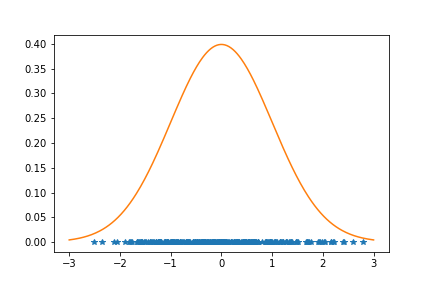
\includegraphics[scale=0.6]{C:/Users/David/Desktop/TFG/TFGLatex/imagenes/normal_01.png}
  \caption[$\mathcal{N}(0,1)$]{Distribución normal de media 0 y desviación típica 1}
  \label{normal_01}
\end{figure}

Esta función será nuestro punto de partida para construir nuestro modelo, el cual asume que las 
características de los datos siguen dicha distribución, es decir, 
$\forall j=1,\cdots,n; \quad x_j \sim \mathcal{N}(\mu_j, \sigma_j^2)$.\\

El objetivo es modelizar una función que denotaremos $p(x)$, que dado un ejemplo, nos devuelva la 
probabilidad de que dicho ejemplo sea anómalo. Más adelante se definirá esta función de manera 
concreta.

Lo primero que debemos hacer es calcular las medias y varianzas de cada característica de nuestros 
ejemplos de entrenamiento (matriz $X$), esto nos da una serie de parámetros 
$\mu = (\mu_1, \ldots, \mu_n) $ y 
$\sigma^2 = (\sigma_1^2, \ldots, \sigma_n^2) $ 
que se utilizaran posteriormente para predecir la probabilidad de que un nuevo dato sea anómalo. 
Mas concretamente:
$$ \mu_j = \frac{1}{m}\sum_{i=1}^{m}x_j^{(i)} \quad 
   \sigma_j^2 = \frac{1}{m}\sum_{i=1}^{m}(x_j^{(i)} - \mu_j)^2 $$

Una vez que tenemos nuestros parámetros calculados ya podemos definir $p(x;\mu,\sigma^2)$ como:
$$ p(x;\mu,\sigma^2) = \frac{1}{\sqrt{2\pi}\sigma}e^{-\frac{1}{2}\frac{x-\mu}{\sigma^2}^2}$$
Esta formula nos da la probabilidad de que un valor de una determinada característica se 
comporte de manera anómala.

\clearpage

Una vez calculadas todas las curvas gaussianas para cada característica del \textit{dataset} definimos $p(x)$ como:
$$ p(x) = \prod_{j=1}^n p(x_j;\mu_j,\sigma_j^2)= p(x_1; \mu_1, \sigma_1^2) \cdots  p(x_n; \mu_n, \sigma_n^2)$$
La función $p(x)$ se comporta como un detector de irregularidades ya que si alguna de las funciones 
$p(x_j;\mu_j,\sigma_j^2)$ para cierto $j$ arroja un valor fuera de lo normal, este quedará reflejado 
en el valor final de $p(x)$.

Llegados a este punto, debemos establecer un cierto umbral $\epsilon$ que nos marque la frontera 
para considerar un ejemplo como normal o anómalo, es decir, marcaremos un ejemplo $x$ como anómalo si 
$p(x)<\epsilon$ y será considerado normal si por el contrario $p(x)>=\epsilon$.
Esta elección del parámetro $\epsilon$ no es algo universal sino que depende del problema en cuestión 
(\autoref{circles_plot}) y el \textit{dataset} utilizado para modelar $p(x)$.
Existen ciertas directrices así como reglas generales para una buena elección de 
$\epsilon$\footnote{\url{https://www.coursera.org/learn/machine-learning/lecture/Mwrni/developing-and-evaluating-an-anomaly-detection-system}}, 
pero están fuera de los objetivos de este documento.
\newline
  
Gráficamente, la función $p(x)$ establece una especie de bola en n dimensiones con un cierto centro 
y radio que dependerá del epsilon elegido y el \textit{dataset} utilizado, en la cual toda representación 
de un ejemplo en el espacio $\mathds{R}^n$ que quede dentro de la bola, será considerado normal, 
si por el contrario dicha representación queda fuera de la bola, entonces será considerado una 
anomalía.

\begin{figure}[h]
  \centering
  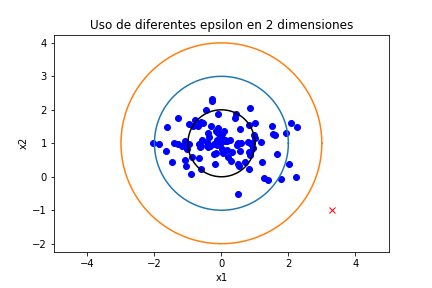
\includegraphics[scale=0.6]{C:/Users/David/Desktop/TFG/TFGLatex/imagenes/circles_plot.png}
  \caption[Ejemplo de anomalía]{Ejemplo de anomalías para distintos valores de $\epsilon$}
  \label{circles_plot}
\end{figure}

En la figura los valores se distribuyen según
$x1 \sim \mathcal{N}(0, 1); \quad x2 \sim \mathcal{N}(1, 0.5)$.
Los círculos concéntricos representan la elección de distintos valores del parámetro $\epsilon$ ,
centrados en el punto $\mu=(\mu_1, \mu_2)=(0, 1)$.
Si tomamos como referencia el circulo mas grande, la $x$ marcada en rojo sería un ejemplo anómalo 
en ese conjunto de datos

\newpage  
  
\subsubsection*{Código MapReduce para el computo de la media y la varianza}
  
\lstinputlisting[caption=ComputeMeanVar.py, language=Python, firstline=10]
                {C:/Users/David/Desktop/TFG/implementaciones/ComputeMeanVar.py}

\begin{lstlisting}[language=bash, numbers=none]
$ python ComputeMeanVar.py <input_file> [-r hadoop]
\end{lstlisting}
%TODO INCLUIR UNA TABLA CON EL DESEMPEÑO DEL ALGORITMO PARA DISTINTOS TAMAÑOS DEL DATASET
  
\newpage

\subsection{K-Means}
\textbf{\textit{K-Means}}\index{K-Means} es uno de los algoritmos de \textit{clusterización}\index{Clusterización} mas 
extendidos y usados en la actualidad. La idea principal del algoritmo es agrupar los datos de entrada 
en distintos conjuntos o \textit{clusters}\footnote{Notese que no se debe confundir el uso de la 
palabra \textit{cluster} para hacer referencia a un \textit{cluster} de maquinas, o cuando se usa 
para referirnos a un conjunto de datos agrupados} 
coherentes, esto es, los puntos dentro de una mismo \textit{cluster} son mas parecidos entre si 
que los puntos de otro \textit{cluster} cualquiera.
\newline

Nuestros datos de entrada son puntos $x^{(i)} \in \mathds{R}^n$ y un cierto numero $k$ de 
\textit{clusters} en los que vamos a agrupar nuestros datos.

Comenzamos estableciendo $k$ puntos en lugares aleatorios de nuestros datos, estos puntos serán los 
centros de los \textit{clusters} $c_1, c_2, \cdots, c_k$, y los llamaremos \textit{centroides}\index{Centroides}.
Una vez hecho esto, el algoritmo recorrerá cada punto $x_i$ y encontrará el centroide $c_j$ mas 
cercano (en términos de la distancia euclídea) a nuestro punto, con lo cual, al punto $x_i$ se le 
asigna el \textit{cluster} $j$.

Una vez que tengamos todos los puntos asignados a sus respectivos centroides mas cercanos, actualizamos 
los centroides con la media de todos los puntos que pertenecen al \textit{cluster} de dicho centroide.

Las iteraciones del algoritmo se detendrán cuando en dos iteraciones sucesivas ninguno de los puntos 
sea asignado a otro \textit{cluster} distinto al anterior o cuando la norma del vector que componen 
la resta de los centroides de dos iteraciones consecutivas sea menos que un cierto $\epsilon$ 
prefijado.
\newline

\noindent \textbf{Pasos del algoritmo K-Means}:
\begin{enumerate}
  \item \textbf{Input}: Puntos en $\mathds{R}^n$ y un numero $k \in \mathds{N}$ de \textit{clusters}
  en los que agrupar nuestros datos.
  \item Insertar $k$ centroides $c_1, c_2, \cdots, c_k$ en localizaciones aleatorias.
  \item Calcular la distancia entre cada punto $x^{(i)}$ y cada centroide $c_i$.
  \item Asignar a cada punto $x^{(i)}$ al \textit{cluster} cuya distancia al centroide sea menor 
        que la distancia al resto de centroides.
  \item Recalcular los nuevos centroides usando la formula $c_i = \frac{1}{m_j} \sum_{j=1}^{m_i}x^{(i)}$ 
        donde $m_i$ es el número de puntos que pertenecen al \textit{cluster} $i$ y $x^{(i)}$ son 
        todos los puntos de dicho cluster, mas concretamente \\
        $x^{(i)} \in \{ p \in \mathds{R}^n \, | \, d(p, c_j) < d(p, c_s) \, \forall s \in 1, \cdots, k; s \neq j \}$.
  \item Calcular la norma entre los centroides anteriores y los nuevos centroides \\
        $ ||(c_1^i, c_2^i, \cdots, c_k^i) - (c_1^{i-1}, c_2^{i-1}, \cdots, c_k^{i-1})||_{\infty} $ 
        donde el superíndice $i$ indica la iteración $i$-ésima.
  \item Si esta norma es menor que un cierto $\epsilon$ prefijado entonces parar, en caso contrario 
        volver al paso $3$        
  \item \textbf{Output}: $k$ centroides $c_1, c_2, \cdots, c_k$.
\end{enumerate}


\begin{figure}[htp]
  \centering
  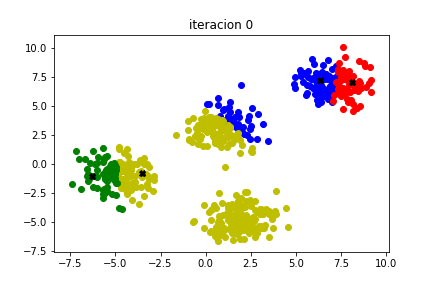
\includegraphics[width=.3\textwidth]{C:/Users/David/Desktop/TFG/TFGLatex/imagenes/kmeans_imagen0.png}\quad
  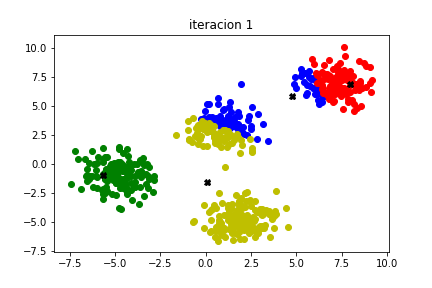
\includegraphics[width=.3\textwidth]{C:/Users/David/Desktop/TFG/TFGLatex/imagenes/kmeans_imagen1.png}\quad
  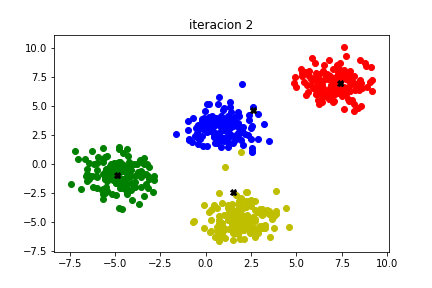
\includegraphics[width=.3\textwidth]{C:/Users/David/Desktop/TFG/TFGLatex/imagenes/kmeans_imagen2.png}

  \medskip

  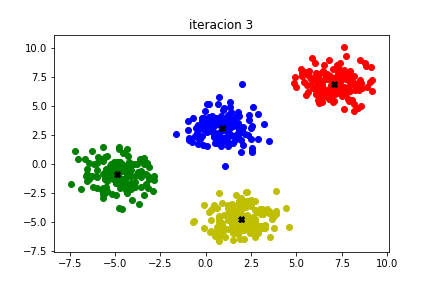
\includegraphics[width=.3\textwidth]{C:/Users/David/Desktop/TFG/TFGLatex/imagenes/kmeans_imagen3.png}\quad
  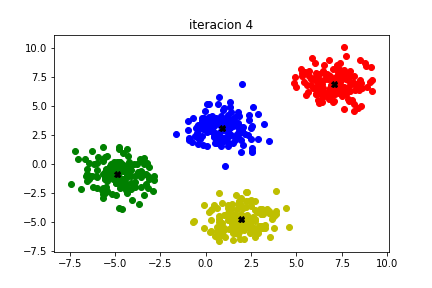
\includegraphics[width=.3\textwidth]{C:/Users/David/Desktop/TFG/TFGLatex/imagenes/kmeans_imagen4.png}

  \caption{Iteraciones del algoritmo k-means}
  \label{kmeans_iteraciones} % para las hyperreferencias
\end{figure}

\newpage

\subsubsection*{Código \textit{Spark} para el algoritmo de \textit{K-Means}}

\lstinputlisting[caption=KMeansSpark.py, language=Python, firstline=8, lastline=72]
                {C:/Users/David/Desktop/TFG/implementaciones/KMeansSpark.py}

\clearpage
Con el fin de testar el código anteriormente escrito:

\lstinputlisting[caption=KMeansMain, language=Python, firstline=74]
                {C:/Users/David/Desktop/TFG/implementaciones/KMeansSpark.py}

\begin{lstlisting}[language=bash, numbers=none]
$ # master puede ser local[*] o yarn-client
$ spark-submit --master yarn-client KMeansSpark.py
\end{lstlisting}

                
%TODO INCLUIR UNA TABLA CON EL DESEMPEÑO DEL ALGORITMO PARA DISTINTOS TAMAÑOS DEL DATASET

\newpage